% CAPITULO 3-------------------------------------------------------------------

\chapter{SEGURANÇA E AUDITORIA}
\label{sec:tarefa3}

A sempre crescente demanda por prestação de mais e melhores serviços públicos tornou
necessário disponibilizar meios de processamento de dados e de comunicação para troca de
informações, bem como para permitir interação entre as organizações públicas e os cidadãos.
Essa interação tem sido mediada cada vez mais pela Internet e por meio de serviços de e-gov
apoiados em sistemas de informação computadorizados. Consequentemente, a segurança (especialmente a disponibilidade, a integridade, a confidencialidade ou sigilo e a autenticidade)
dessas informações passou a ser uma preocupação do poder público e um tema crítico da
gestão moderna, seja ela pública ou privada. Uma forma de gerenciar essa criticidade é criar
normas, formular políticas, padronizar procedimentos e práticas, estabelecer medições e métricas, além de automatizar controles, de modo a não só aumentar previsibilidade dos resultados dessa prestação de serviço, mas principalmente melhorar a capacidade de lidar com riscos
decorrentes das vulnerabilidades dos sistemas – sejam eles manuais ou automatizados - e das
ameaças existentes (sobretudo as originadas da Internet).

Essas normas, políticas, procedimentos, práticas, métricas e mecanismos automatizados
são controles, e podem ser analisadas através de sua vinculação com os objeto de controle
que são decompostos em pontos de controle. A auditoria de segurança de informação é uma
atividade devidamente estruturada para examinar criteriosamente a situação desses controles
que se aplicam à segurança da informação, especialmente por meio da análise de objetos e
seus pontos de controle, vis-a-vis a probabilidade de ameaças às informações críticas sobre as
quais atuam esses controles. Isto é necessário porque os controles ou a ausência deles podem
se constituir em vulnerabilidades exploráveis ou portas de entrada para produzir incidentes
de segurança da informação. A auditoria cria condições técnicas para investigar e emitir um
juízo sobre as evidências encontradas, de modo a se antecipar ante a possíveis riscos de violação de um patrimônio precioso: os ativos de informação. Esses ativos correspondem àquelas
informações e todos os recursos associados que têm alto valor para o negócio público ou privado. Consideram-se como ativos de informação os processos organizacionais e processuais
(procedimentos, roteiros, atividades), itens físicos (instalações, equipamentos, cabeamento) e
lógicos (programas, sistemas, estruturas de dados), que devem ser auditados continuamente.

De outra forma, auditoria é a expressão de opinião feita por um profissional devidamente
qualificado, acerca de uma determinada situação, e documentada na forma de um relatório
ou parecer. Para tal, o auditor emprega práticas geralmente aceitas, baseadas em um método
racional, em evidências, em respeito aos princípios éticos, com responsabilidade perante o
cliente, com devido cuidado e habilidade profissional, sujeito à revisão por pares, mas com
independência no que se refere à roteirização, à investigação e análise e à produção do relato.

Em linhas gerais, a auditoria de segurança da informação pretende assegurar que os ativos de informação, considerados os objetos de auditoria em segurança da informação, estejam absolutamente sob controle da organização. Para tal, é preciso verificar que os controles
estejam de acordo com as normas e políticas de segurança estabelecidas para esses ativos,
bem como se o que está em operação alcança os objetivos de segurança definidos. A auditoria
de segurança de informação envolve também o provimento de uma avaliação independente
dos controles da organização (normas, políticas, padrões, procedimentos, práticas, métricas
e mecanismos) empregados para salvaguardar a informação, em formato eletrônico ou não,
contra perdas, danos, divulgação não intencional e indisponibilidades. Por fim, a auditoria é
uma atividade realizada na forma de ações projetizadas, que tem um início, meio e fim, e que
visam produzir resultados dentro de custos, prazos e qualidades esperadas. Para alcançar tais
objetos, as auditorias, projetos individuais, agrupam-se em programas, que compreendem a
realização de várias auditorias ao longo de um período de tempo de meses ou anos, e que
visam melhorar sistematicamente o desempenho, a eficiência e a segurança organizacionais.

\nocite{auditoria}

\section{Teste de Software}

Teste de software é o processo de execução de um produto para determinar se ele atingiu suas especificações e funcionou corretamente dentro do ambiente para o qual foi projetado.
O seu objetivo é buscar falhas em um produto, para que as causas dessas falhas sejam identificadas e possam ser corrigidas pela equipe de desenvolvimento antes da entrega final.

\subsection{Teste caixa-branca (ou Teste Estrutural)}

Teste de caixa branca é a técnica de teste que testa a estrutura interna e a implementação do produto, tornando-as visíveis para o testador. Aqui, a estrutura interna implica design, código, fluxo de dados e bancos de dados. O objetivo do teste de caixa branca é verificar o fluxo de trabalho interno do produto. A eficácia dos testes é medida por meio da cobertura de código. Para definir, a cobertura de código é a porcentagem de linhas de código exercidas por meio dos testes do total de linhas de código. Os outros nomes comuns para o teste de caixa branca são caixa transparente, caixa de vidro, caixa transparente ou teste estrutural.

A realização de testes de caixa branca requer programação, banco de dados e conhecimento de design do produto. Além disso, os testadores também exigem o conhecimento de ferramentas como ferramentas de cobertura e depuradores para testes de caixa branca.

O exemplo típico de teste de caixa branca é o teste de componentes do produto. Por definição, Teste de componentes significa testar as unidades de componentes individuais do produto, que podem ser um único programa ou grupo de programas formando um módulo. Assim, esses testes se concentram na avaliação daquele módulo específico. Pode-se escrever testes \textit{JUnit} ou \textit{Cucumber} para este tipo de teste de componentes. Normalmente, esses testes invocam métodos ou funções que fornecem os dados de entrada e avaliam sua saída comparando-os com os resultados esperados.

\nocite{branca}
\nocite{testeufpr}

\subsection{Teste caixa-preta (ou Teste Funcional)}

Técnica de teste em que o componente de software a ser testado é abordado como se fosse uma caixa-preta, ou seja, não se considera o comportamento interno do mesmo.
Dados de entrada são fornecidos, o teste é executado e o resultado obtido é comparado a um resultado esperado previamente conhecido.
Haverá sucesso no teste se o resultado obtido for igual ao resultado esperado.
O componente de software a ser testado pode ser um método, uma função interna, um programa, um componente, um conjunto de programas e/ou componentes ou mesmo uma funcionalidade.

\nocite{canaltiteste}

\subsection{Teste caixa-cinza}

O teste de caixa cinza é um tipo de teste profissional frequentemente usado para software de computador, que combina certos aspectos do teste de caixa preta e teste de caixa branca. A idéia geral é combinar esses dois outros tipos para utilizar os pontos fortes de cada um, minimizando suas limitações ou fraquezas. O teste da caixa cinza consiste basicamente em testes profissionais, nos quais os testadores compreendem algumas das maneiras pelas quais o software funciona, mas eles não entendem tudo sobre ele.

Ao desenvolver e testar software de computador, existem dois modelos comuns de teste frequentemente utilizados. São testes de caixa preta e de caixa branca, e o teste de caixa cinza é basicamente uma combinação de ambos. O teste da caixa preta consiste em testes nos quais os testadores não entendem ou têm acesso ao código que executa o software. Por exemplo, alguém pode utilizar o teste de caixa preta para permitir que uma empresa externa desenvolva software para executar com um sistema operacional (SO) sem fornecer à empresa o código fonte do SO.

Esse tipo de teste é frequentemente usado por muitas empresas de \textit{software} e pode ser usado para testes internos e externos. Uma das maiores fraquezas desse tipo de teste, no entanto, é que o conhecimento limitado dos testadores pode potencialmente dificultar seus testes. O teste de caixa cinza procura aliviar alguns desses problemas combinando esse tipo de teste com certos elementos do teste de caixa branca.


O teste de caixa branca consiste em testes de software realizados por pessoas que compreendem completamente o software que está sendo testado e têm acesso ao código-fonte do software. Isso geralmente é feito internamente em um desenvolvedor de software para garantir que o programa funcione corretamente e para permitir que os testadores interajam diretamente com o código por trás do programa. Porém, existem problemas de segurança em potencial com esse tipo de teste e, portanto, o teste da caixa cinza é frequentemente usado para combinar os dois tipos de maneira produtiva e segura.

No teste da caixa cinza, os testadores compreendem certos aspectos do software que está sendo usado e podem ver algumas partes do código-fonte, mas não todo. Isso permite que os testadores interajam e compreendam mais completamente o programa que estão testando do que o teste de caixa preta permite, mas sem os problemas completos de acesso e segurança que podem surgir dos testes de caixa branca. Alguém que esteja realizando testes de caixa cinza no software de um novo sistema operacional, por exemplo, poderá ver o código de aspectos do sistema operacional relevantes para o teste do programa, mas não todo o código-fonte.

\begin{figure}[H]
    \centering
    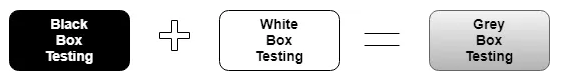
\includegraphics[width=0.7\linewidth]{dados/figuras/grey}
    \caption{Teste Caixa Cinza}
    \label{fig:teste}
\end{figure}

